\documentclass{article}
\usepackage{float}
\usepackage{wrapfig}
\usepackage[font=footnotesize]{caption}
\usepackage{amsmath}
\usepackage{listings}
\usepackage{xcolor}
\usepackage{graphicx}
\usepackage{enumitem}
\usepackage{hyperref}
\usepackage[bottom]{footmisc}
\setlength{\footnotesep}{\baselineskip}

\title{PHYS 605 Lab 3 Analog 2 Progress Report}
\author{Name: Dan Albu\thanks{Each reference used in this report is a hyperlink.} \\Lab Partner: Ryan Coyne}
\date{March 1, 2024}

\begin{document}

\maketitle
\section{Introduction}
In this lab, we learned about impedance, RC, and RLC circuits. We also learned how to create Bode and Gain\footnote{Gain plots will be interchangeably reffered to as Attenuation plots throughout the report} plots. In addition to this, we became more familiar with the oscilloscope and function generator, as well as how different frequencies interact with different circuits, such as the high pass and low pass circuits.

\subsection{Equipment Used}
\begin{itemize}[label=--]
    \item \textbf{Mastech MS8268 Multi-Meter}
        \begin{description}
            \item[$\circ$ NOTE:]Referenced as Multi-meter, Ohmmeter, Voltmeter, or Ammeter
        \end{description}
    \item \textbf{PB-503 Proto-board}
        \begin{description}
            \item[$\circ$ NOTE:]Referenced as board or breadboard
        \end{description}
    \item \textbf{Analog Discovery 2 - USB Oscilloscope and Signal Generator}
        \begin{description}
            \item[$\circ$ NOTE:]Referenced as AD, Analog Discovery, Oscilloscope, Scope, WaveGen, or wave generator\footnote{ The Analog Discovery can also act as an Ammeter or Voltmeter. If it is being mentioned, it will be noted that it is the AD rather than the Mastech MS8268. If both are being used, the AD instrument will have an * symbol after it to differentiate between the two.}
        \end{description}
    \item[] \vspace{10mm}
    \item[$\bullet$] \textbf{Components \footnote{Not including the capacitors used for testing capacitance}}
        \begin{description}
            \item[$\circ$] 100 nF Capacitor
            \item[$\circ$] 10 k$\Omega$ Resistor
            \item[$\circ$] 1 mH Inductor
        \end{description}
\end{itemize}
\begin{table}[h!]
    \centering
    \begin{tabular}{|c|c|}
        \hline
        Capacitor Value & Associated ID (Front/Back)\\
        \hline
        10 nF & 103CSK/531RFO\\
        \hline
        100 nF & 104ESM/335ACA\\
        \hline
        1 $\mu$F & BCI052\protect\footnotemark\\
        \hline
    \end{tabular}
    \caption{Capacitor Identification}
    \label{tab:Capacitor Identification}
\end{table}
\footnotetext{This may have been BC105Z but unfortunately my handwriting does not allow one to discern between the two.}
\subsection{Help}
\begin{itemize}
    \item{\fontsize{11pt}{13.6pt}\selectfont Who we helped}
    \begin{itemize}[label=$\circ$]
        \item Conor Bosworth's Group located in front of us
        \item Ryan McClennan and Audrey Robison's group located behind us
    \end{itemize}
    \item{\fontsize{11pt}{13.6pt}\selectfont Who helped us}
    \begin{itemize}[label=$\circ$]
        \item Dr. Holtrop and Gavin Riley
    \end{itemize}
\end{itemize}

\section{Measuring Capacitance}
\vspace{-1mm}
\begin{wrapfigure}[11]{r}{0.5\textwidth}\vspace{-5mm}
    \centering
    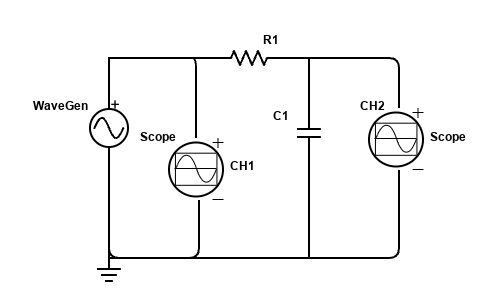
\includegraphics[width=0.5\textwidth]{Images/Scheme-it-export-PHYS-605-L3A2-Low-Pass-2024-03-02-22-46.png}
    \caption{Low Pass Circuit Schematic}
    \label{fig:Low Pass Circuit}
\end{wrapfigure}
Before we started analyzing low and high pass circuits, we had to verify the capacitance of the capacitors we were using. To do this, we first built a low pass circuit (Figure \ref{fig:Low Pass Circuit}). We made sure to connect channel 1 of the oscilloscope in parallel with the WaveGen to plot the 1 $V$ square wave output of the WaveGen. After connecting a resistor in series with the WaveGen then adding a capacitor, we added channel 2 of the oscilloscope in parallel with the capacitor to plot the voltage across the capacitor, which can also be modelled as the output voltage of the circuit. We gathered three different capacitors: 10 nF, 100 nF, and 1 $\mu$F. We then had to choose three resistor values to use with the capacitors. We chose 100 k$\Omega$, 10 k$\Omega$, and 1 k$\Omega$ resistors, corresponding to the 10 nF, 100 nF, and 1 $\mu$F capacitors respectively. After circuit was built, we used a square wave with an amplitude of 0.5 $V$ centered at 0 $V$ and four different frequencies to measure the capacitance of the capacitors using the ``Impedance" measurement on the AD. The frequencies used were 1 kHz, 500 Hz, 200 Hz, and 100 Hz. We then used the Mastech MS8268 Multi-meter to measure the capacitance of each capacitor and compared values.

\subsection{Data}

\begin{table}[h!]
    \centering
    \begin{tabular}{|c|c|c|c|}
        \hline
        Frequency (Hz) & 10 nF & 100 nF & 1 $\mu$F\\
        \hline
        1000 & 9.16 nF & 89.2 nF & 1.05 $\mu$F\\
        \hline
        500 & 9.21 nF & 90.1 nF & 1.08 $\mu$F\\
        \hline
        200 & 9.29 nF & 91.3 nF & 1.15 $\mu$F\\
        \hline
        100 & 9.34 nF & 92.1 nF & 1.19 $\mu$F\\
        \hline
    \end{tabular}
    \caption{Analog Discovery Expected Capacitance vs Measured Capacitance per Frequency}
    \label{tab:AD Capacitance Measurements}
\end{table}
\begin{table}[h!]
    \centering
    \begin{tabular}{|c|c|}
        \hline
        Expected Capacitance & Measured Capacitance\\
        \hline
        10 nF & 9.2 nF\\
        \hline
        100 nF & 90.6 nF\\
        \hline
        1 $\mu$F & 1.13 $\mu$F\\
        \hline
    \end{tabular}
    \caption{Multi-meter Expected Capacitance vs Measured Capacitance}
    \label{tab:MM Capacitance Measurements}
\end{table}
\subsection{Conclusion}
We determined that the AD was a much more trustworthy measurment device, as its measurements were much closer for almost every measurement. However we determined that the Multi-meter was still useful for a quick, less accurate measurement. An interesting thing we noted was that the capacitance had an inversely proportional dependence the frequency of the input signal. This is something we had already learned from the equations:
\begin{align}
    Z_C = \hspace*{1mm}\hspace*{1mm}\frac{1}{j\omega C}\Rightarrow&\hspace*{2mm}
    C = \hspace*{1mm}\frac{1}{j\omega Z_C}\\
    C \propto \hspace*{1mm}&\hspace*{1mm}\frac{1}{\omega}
    \label{eq:Impedance of a Capacitor}
\end{align}
but it was interesting to see this relationship with data.

\section{Low Pass Filter Circuit}
\subsubsection*{NOTE}
During this lab my lab partner and I were under the impression that Attenuation plots and Bode plots were the same thing due to misinterpretting the directions at the beginning of the lab and thus did not gather data for the Attenuation plots. We did, however, gather data for the Bode plots. Since we have the data for the Bode plots, we used that data to make the Attenuation plots. We used:
\begin{equation}
    B = 20log(\frac{V_{out}}{V_{in}})\\
\end{equation}
and since we know that Attenuation, or Gain is just $V_{out}/V_{in}$, we can use the equation for $B$ to get the equation for Gain, $G$:
\begin{align}
    \frac{B}{20} = log(\frac{V_{out}}{V_{in}})\text{ } \Rightarrow \text{ } 10^{\frac{B}{20}} = \frac{V_{out}}{V_{in}}
\end{align}
thus we get:
\begin{equation}
    G = 10^{\frac{B}{20}}\label{eq:Gain}
\end{equation}
So in the plotting program I divided every value in the Bode plot data array by 20 and raised it to the exponent with 10 as the base to get the Gain plot data array.

\subsection{Low Pass Filter}
\begin{wrapfigure}[13]{r}{0.6\textwidth}
    \centering
    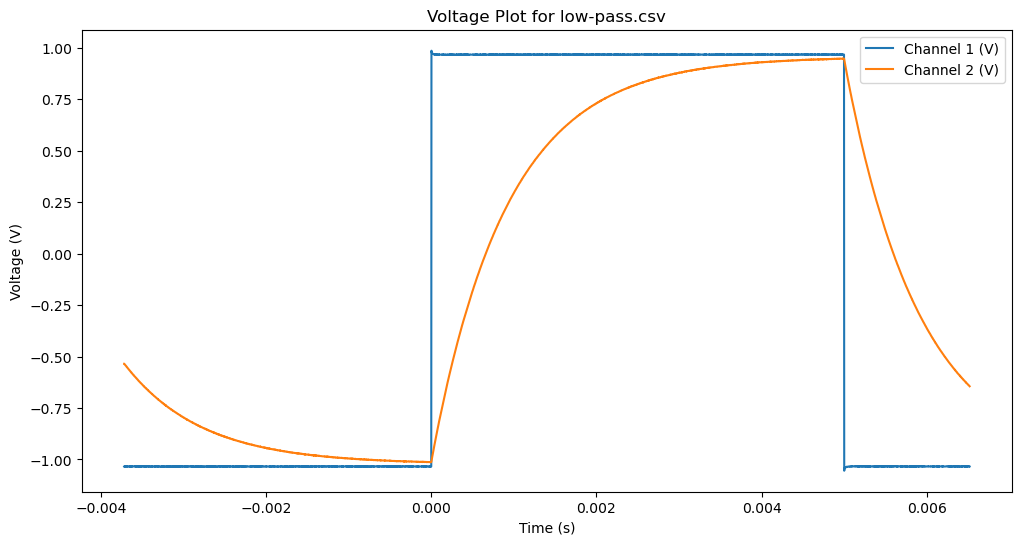
\includegraphics[width=0.6\textwidth]{Images/low-pass-voltage.png}
    \caption{Low Pass Voltage Plot}
    \label{fig:Low Pass Voltage Plot}
\end{wrapfigure}
Now, after determining our capacitance and the accuracy of our measuring devices, we would start analyzing the low pass filter in earnest. Using the same circuit (Figure \ref{fig:Low Pass Circuit}) as before, our resistor value was 10 k$\Omega$ and our capacitor value was 100 nF. Our input was a square wave at 100 Hz, with an amplitude of 1 V, centered at 0 V with a total $\Delta$V of 2 V. Our time position was 0 s and our base was 2 ms/div. Our range for both channel 1 \& 2 was 500mV/div, with a 0 V offset. Our plot of the input voltage (Channel 1) and the output voltage (Channel 2) can be seen in Figure \ref{fig:Low Pass Voltage Plot}. After using the AD to get the measurements for rise ($t_R$) and fall ($t_F$) time, we used our cursor measurement to measure the time it took for the voltage to go from 1 V to $e^{-1}$ V and $e^{-2}$ V respectively (marked as $t_1$ and $t_2$ in equation \ref{eq:time1} and \ref{eq:time2}). Once we had these measurements, we used each of these times to calculate the capacitance of the capacitor. We then compared each of these values to the expected capacitance of the capacitor to determine which was the most accurate. To calculate the values seen in Table \ref{tab:Low Pass Filter Capacitance Calculations}, we used the equation for the fall time: 
\begin{equation}
    V(t) = V_0e^{\frac{-t}{RC}}\\
\end{equation}
solving for C we get:
\begin{equation}
    C = \frac{t}{Rln(\frac{V_0}{V(t)})}
\end{equation}
and with the initial conditions:
\begin{equation}
    \text{ } V_0 = 1 V, \text{ } V(t_1) = e^{-1} V, \text{ } V(t_2) = e^{-2} V
\end{equation}
we get:
\begin{equation}
    C_1 = \frac{t_1}{R}, \text{ } C_2 = \frac{t_2}{2R}\label{eq:Capacitance Calculations}
\end{equation}
Since the capacitance is the same regardless of whether we use the rise time or fall time equation, we used the fall time equation to calculate our capacitance using both $t_R$ and $t_F$ since it was more simple. When calculating these values in lab, I made a good amount of math errors, so in this report I am making sure to rectify those errors and present the corrected data and calculations (Table \ref{tab:Low Pass Filter Capacitance Calculations}). To calculate the capacitance with $t_R$ and $t_F$ we used:
\begin{equation}
    V(t_F) = V_0e^{\frac{-t}{RC}} 
\end{equation}
In the case for rise and fall time, we know that regardless of which equation we use, our equation will simplify to the same point, so we will solve the equation for the case of fall time; that is, for when $V(t) = 0.9V_0$ and $V_0 = 1 V$. This gives us:
\begin{align}
    V(t_F) = 0.9V_0 = V_0e^{\frac{-t_F}{RC}} \Rightarrow& 0.9 = e^{\frac{-t_F}{RC}} \Rightarrow ln(0.9) = \frac{-t_F}{RC}\label{eq:Voltage fall time}\\
    C_F =& \frac{t_F}{Rln(9)}\label{eq:Capacitance fall time}
\end{align}
Where we can substitute $t_R$ into $C_F$ for  $C_R$. We can then use Equation \ref{eq:Capacitance fall time} and compute capacitance values. Of all the values we computed(Table \ref{tab:Low Pass Filter Capacitance Calculations}), the value from the rise time seemed the most trustworthy\footnote{The fall time is a close second place.} as it was the closest in value to the expected 100 nF capacitor we used as seen from the error row. After this we created a Bode plot with a Phase plot(Figure \ref{fig:Low Pass Bode Plot}), plotting Gain (dB) vs Frequency (Hz) and Phase (degrees) vs Frequency (Hz) for the low pass filter. Using Equation \ref{eq:Gain} we also made an Attenuation plot(Figure \ref{fig:Low Pass Gain plot}), plotting Magnitude (x) vs Frequency (Hz) Our frequency range was 20 Hz to 200 kHz for all three plots. We also plotted the square wave input and circuit's output as shown in Figure \ref{fig:Low Pass Voltage Plot}. The Voltage plot is very clean and is exactly what we saw on the WaveForms software. We can see that it starts at 0 degrees and falls down near $-$90. With the low pass filter, the voltage plot shows a visual representation for the capacitor charging up and discharging as voltage is applied by the square wave input. Our Bode plot was also quite good once I made the x-axis logarithmic, but has some noise in the higher frequencies. The Phase plot had the most notable noise of the three plots, but it was still quite accurate to what we saw on the WaveForms software. The Gain plot was the cleanest, even though I expected there to be some artifacting or noise due to the calculations I had to do to get the data for the plot.
\subsection{Data and Calculations}
\begin{align}
    \text{Time from 1 V to $e^{-1}$ V: }&t_1 = 1.5 \text{ ms}\label{eq:time1}\\
    \text{Time from 1 V to $e^{-2}$ V: }&t_2 = 2.3 \text{ ms}\label{eq:time2}
\end{align}
\begin{table}[h!]
    \centering
    \begin{tabular}{|c|c|c|c|}
        \hline
        Rise Time ($t_R$) & Fall Time ($t_F$) & $t_1$ & $t_2$\\
        \hline
        1.97 ms & 1.96 ms & 1.5 ms & 2.3 ms\\
        \hline
    \end{tabular}
    \caption{Low Pass Filter Rise and Fall Times}
    \label{tab:Low Pass Filter Times}
\end{table}

\begin{table}[h!]
    \centering
    \begin{tabular}{|c|c|c|c|}
        \hline
        $C_R$ & $C_F$ & $C_1$ & $C_2$\\
        \hline
        89.64 nF & 89.18 nF & 150 nF & 115 nF\\
        \hline
        10.36\% & 10.82\% & 50\% & 15\%\\
        \hline
    \end{tabular}
    \caption[Low Pass Filter Capacitance Calculations using Equations \ref{eq:Capacitance Calculations} and \ref{eq:Capacitance fall time} with Error]{Low Pass Filter Capacitance Calculations using Equations \ref{eq:Capacitance Calculations} and \ref{eq:Capacitance fall time} with Error\footnotemark}
    \label{tab:Low Pass Filter Capacitance Calculations}
\end{table}
\footnotetext{The error is calculated using: $\text{Error} = \lvert\frac{\text{Measured $-$ Expected}}{\text{Expected}}\rvert \times 100\%$}
\vspace{-3mm}
\begin{figure}[h!]
    \centering
    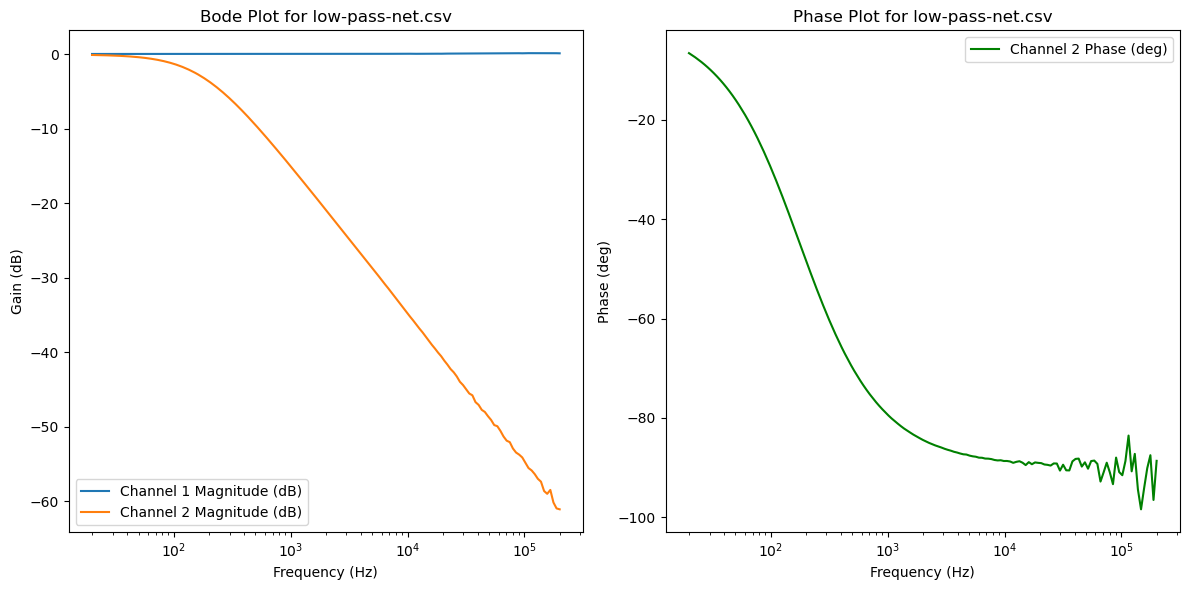
\includegraphics[width=0.8\textwidth]{Images/low-pass-bode.png}
    \caption{Low Pass Bode and Phase Plot}
    \label{fig:Low Pass Bode Plot}
\end{figure}
\vspace{-5mm}
\begin{figure}[H]
    \centering
    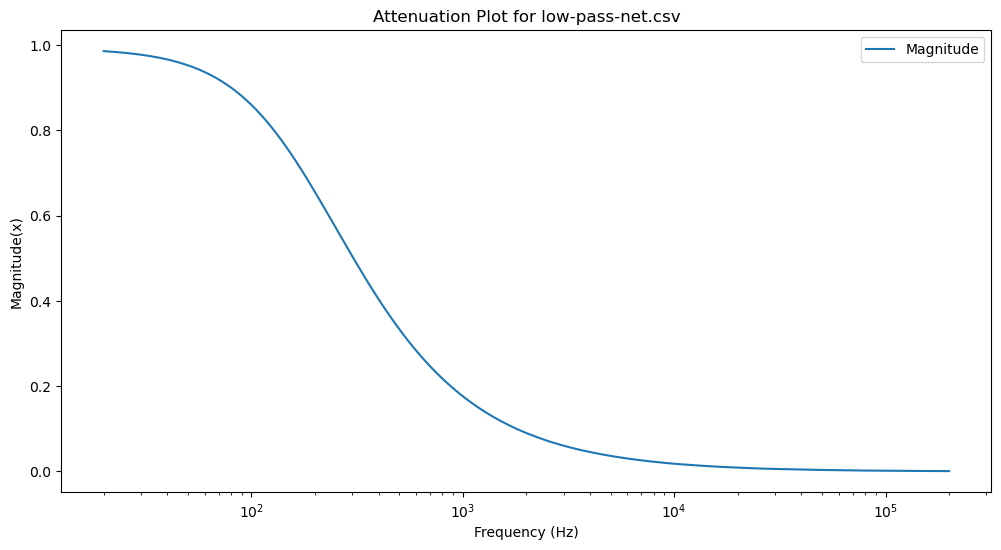
\includegraphics[width=0.7\textwidth]{Images/low-pass-gain.png}
    \caption{Low Pass Gain plot}
    \label{fig:Low Pass Gain plot}
\end{figure}
\vspace{-5mm}
\subsection{Conclusion}
We learned that the rise and fall time calculated by the AD were the most accurate, giving us a more accurate capacitance measurement. The Bode plot shows how the signal's strength behaves as a function of frequency. For the Low Pass Filter, the signal attenuates with higher frequencies. The Phase plot shows how the phase of the signal behaves as a function of frequency. For the Low Pass Filter, the phase of the signal is near 0 degrees at lower frequencies, and approaches $-$90 degrees as the frequency increases. Around the cutoff frequency, the Phase plot seems to slow down, that is, $\frac{d\phi}{d\omega}$ decreases after the cutoff frequency\footnote{It looks like the cutoff frequency could also be described by where $\frac{d^2\phi}{d\omega^2} = 0$, as it looks like the cuttoff frequency is at the inflection point but this is just speculation.}.A good reason to make such a circuit would be to limit specific frequencies, which in terms of applications, could be used for a multitude of things, such as audio filters, regulating voltage, and even in radio communications. The Attenuation plot shows very clearly, in terms of magnitude, the ``strength'' of the signal; giving the viewer an intuitive and useful way to see how the signal behaves as a function of frequency. 
\vspace{-3mm}
\section{High Pass Filter Circuit}
\begin{wrapfigure}[11]{r}{0.6\textwidth}\vspace{-9mm}
    \centering
    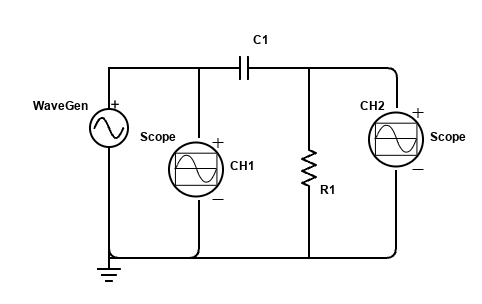
\includegraphics[width=0.6\textwidth]{Images/Scheme-it-export-PHYS-605-L3A2-High-Pass-2024-03-03-23-32.png}
    \caption{High Pass Circuit Schematic}
    \label{fig:High Pass Circuit}
\end{wrapfigure}

For the high pass filter we were instructed to repeat the same steps as with the low pass, so to make this section more compact, you can assume that everything that is not mentioned here was done and had the same result as the low pass circuit unless mentioned otherwise. Our high pass circuit was built through modifying our low pass circuit from the previous section by just switching the resistor and capacitor, as shown in Figure \ref{fig:High Pass Circuit}. All of our components are the same; therefore, we can do our calculations without much changing. We gathered our data by using the same square wave input as before at the same frequency, 100 Hz, and plotted the input and output voltages, marked as channels 1 and 2 on Figure \ref{fig:High Pass Voltage Plot}.
\begin{wrapfigure}[11]{l}{0.5\textwidth}
    \centering
    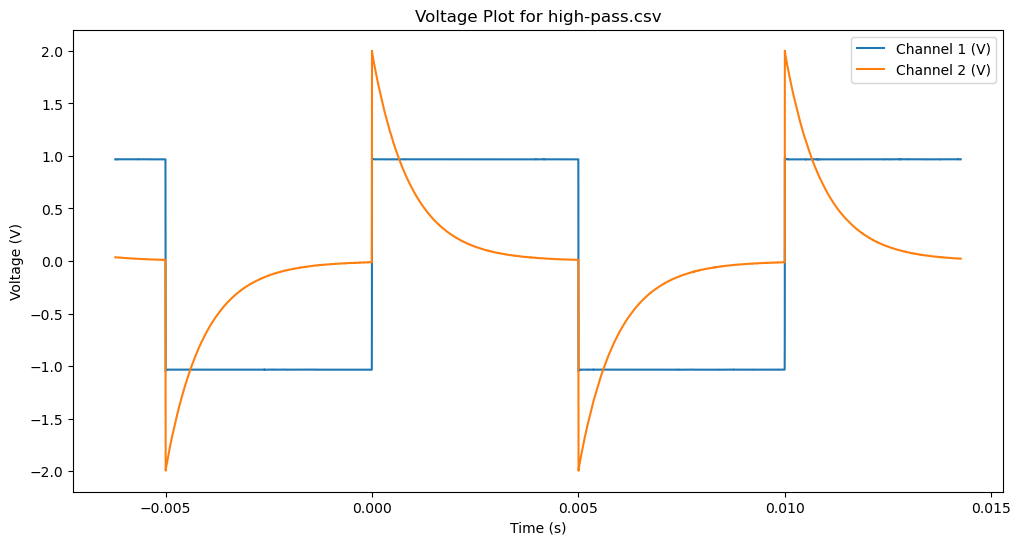
\includegraphics[width=0.5\textwidth]{Images/high-pass-voltage.png}
    \caption{High Pass Voltage Plot}
    \label{fig:High Pass Voltage Plot}
\end{wrapfigure}

\noindent We can see that instead of the output being smaller that the input, we can see the capacitor charging at the beginning of the square wave and discharging as the wave continues. Our measurements for our rise and fall time are different(Table \ref{tab:High Pass Filter Times}) but the equations we used to calculate the capacitance are the same(Equations \ref{eq:Voltage fall time} and \ref{eq:Capacitance fall time}). During the lab, we didn't actually get the times for the voltage to fall from 1 V to $e^{-1}$ V and $e^{-2}$ V, so I relied on the workspace that my partner Ryan sent me. Unfortunately, my WaveForms software doesn't recognize the file as a workspace, so I do not have data for those times. I will still do the calculations for the rise and fall time(Table \ref{tab:High Pass Filter Capacitance Calculations}), but unfortunately I will not be able to compare the calculated capacitance from the rise and fall time to the data from the high pass circuit's $t_1$ and $t_2$. Using the results from Table \ref{tab:High Pass Filter Capacitance Calculations}, we find that rise time is the most accurate for calculating capacitance as it is closer to the expected value, 100 nF. Even though I don't have $t_1$ or $t_2$, the method of data acquisition for those values is less accurate than the AD's rise and fall time values as it relies on getting the approximate value of $e^{-1}$ and $e^{-2}$ with the cursor. Interestingly, the Bode and Phase plot (Figure \ref{fig:High Pass Bode Plot}) as well as the Gain plot (Figure \ref{fig:High Pass Gain Plot}) for the high pass circuit were much better than the plots for the low pass circuit. 

\subsection{Data and Calculations}
\begin{table}[h!]
    \centering
    \begin{tabular}{|c|c|}
        \hline
        Rise Time ($t_R$) & Fall Time ($t_F$) \\
        \hline
        2.86 ms & 3.01 ms\\
        \hline
    \end{tabular}
    \caption{High Pass Filter Rise and Fall Times}
    \label{tab:High Pass Filter Times}
\end{table}
\begin{table}[h!]
    \centering
    \begin{tabular}{|c|c|}
        \hline
        $t_R$ & $t_F$\\
        \hline
        130.16 nF & 139.99 nF\\
        \hline
        30.16\% & 39.99\%\\
        \hline
    \end{tabular}
    \caption{High Pass Filter Capacitance Calculations using Equation \ref{eq:Capacitance fall time} with Error}
    \label{tab:High Pass Filter Capacitance Calculations}
\end{table}
\begin{figure}[h!]
    \centering
    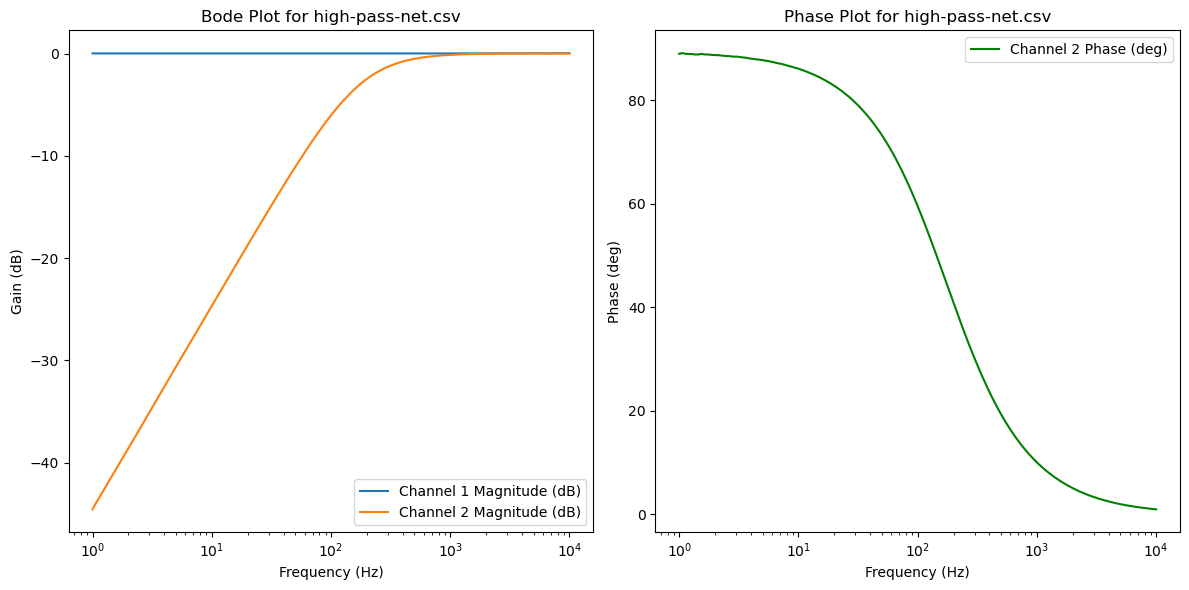
\includegraphics[width=0.8\textwidth]{Images/high-pass-bode.png}
    \caption{High Pass Bode and Phase Plot}
    \label{fig:High Pass Bode Plot}
\end{figure}
\begin{figure}[H]
    \centering
    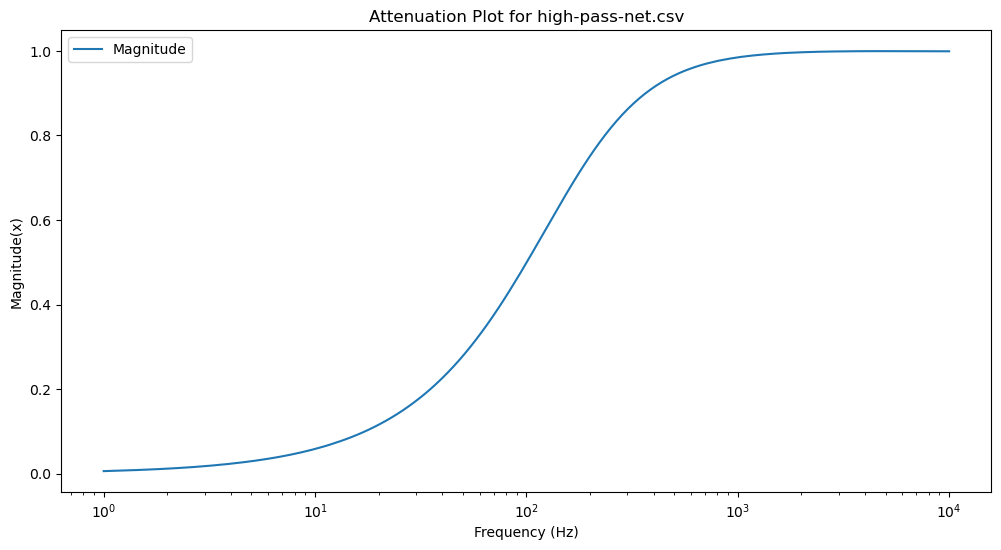
\includegraphics[width=0.7\textwidth]{Images/high-pass-gain.png}
    \caption{High Pass Gain Plot}
    \label{fig:High Pass Gain Plot}
\end{figure}
\subsection{Conclusion}
For the high pass filter, it seems like the rise and fall times we recorded resulted in a calculation that was greater than the expected capacitance rather than less than like the low pass filter. As seen from the error row in Table \ref{tab:High Pass Filter Capacitance Calculations}, $t_R$ is more accurate than $t_F$. We can see that for the high pass filter, the Bode plot starts at a much lower value than the low pass filter, and and rises in the same fashion as the low pass filter's Bode plot. The Phase plot for the high pass filter is very similar to the low pass filter's but instead of starting at 0 degrees and ending to $-$90, it starts at  90 degrees and falls to 0 degrees. The Gain plot is very similar to the low pass filter's, but it is inverted across the y-axis. A high pass filter would definitely be useful in the same way as a low pass filter, though naturally used for different applications. For example, a high pass filter could be used to remove low frequency noise from a signal, or to remove DC offset from a signal.
\vspace{-5mm}
\section[RLC]{RLC Band-Pass Flter Circuit\footnote{We skipped the inductor part as we were running low on time and were more interested in the RLC band-pass filter.}}
\begin{wrapfigure}[12]{r}{0.6\textwidth}\vspace{-5mm}
    \centering
    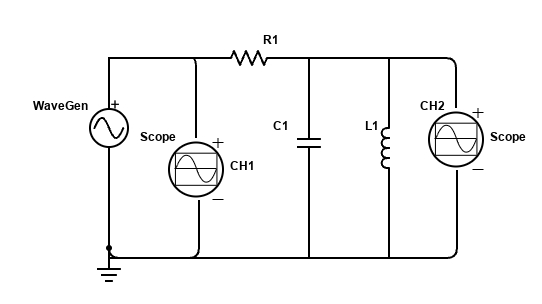
\includegraphics[width=0.6\textwidth]{Images/Scheme-it-export-PHYS-605-L3A2-RLC-Band-Pass-2024-03-03-23-39.png}
    \caption{RLC Band-Pass Circuit Schematic}
    \label{fig:RLC Circuit}
\end{wrapfigure}
The last part of the lab was to analyze a low pass circuit with an inductor in parallel with the capacitor, as shown in Figure \ref{fig:RLC Circuit}. For our RLC band-pass filter, we used the same resistor and capacitor as the low pass and high pass filters, but we used a 1 mH inductor. The components we used worked well allowing us to observe resonance in the form of the ringing signal. We used the same square wave input as before at the same frequency, 100 Hz, and measured the ringing frequency ($f_r$) and its corresponding $\Delta t$(Table \ref{tab:RLC freq}). After this we made a Bode plot with a Phase plot(Figure \ref{fig:RLC Bode Plot}) and a Gain plot(Figure \ref{fig:RLC Gain Plot}) using the data from the circuit. These plots were radically different from the low and high pass filters. As the name ``Band-Pass'' suggests, there is a band of frequencies that isn't attenuated. This is most easily observed in the Gain plot, since it's y-axis isn't logarithmic it can be much easier to visualize where the band is. The Bode plot had some noise around the lower and higher frequencies, which was only accentuated in the the Phase plot, which has a much different shape than the previous ones, ranging from 90 to $-$90, with a steep drop around 16 kHz. Each plot clearly has an interesting point at the ringing frequency, with the Phase plot having a steep drop and the Gain and Bode plot having peaks at that point.
\subsection{Data}
\begin{figure}[h!]
    \centering
    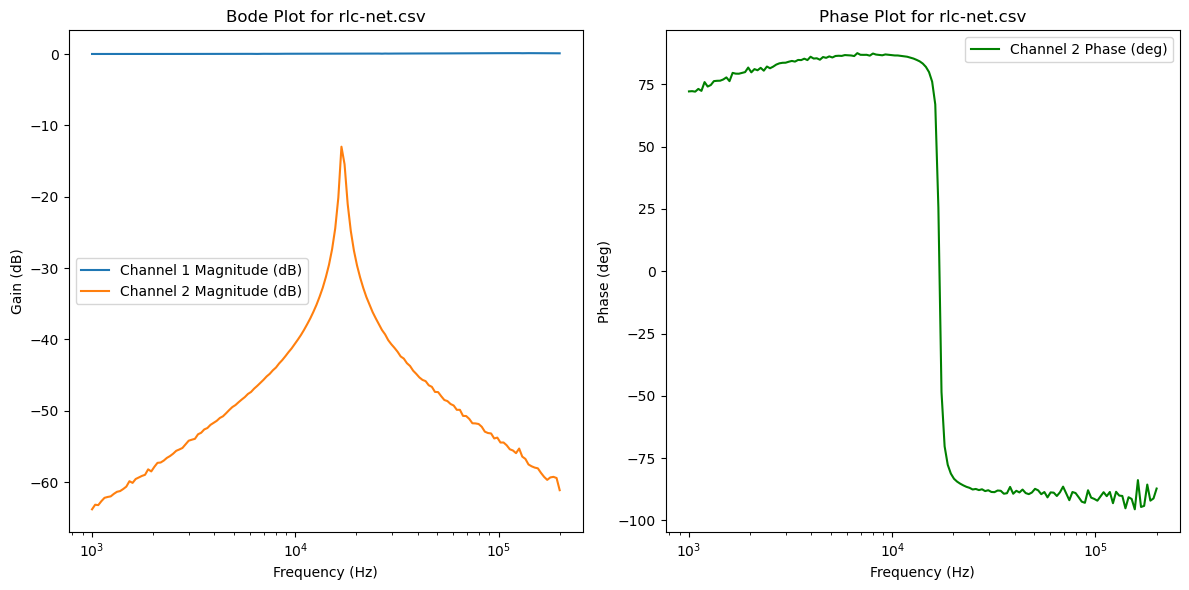
\includegraphics[width=0.75\textwidth]{Images/rlc-bode.png}
    \caption{RLC Band-Pass Bode and Phase Plot}
    \label{fig:RLC Bode Plot}
\end{figure}
\begin{figure}[H]
    \centering
    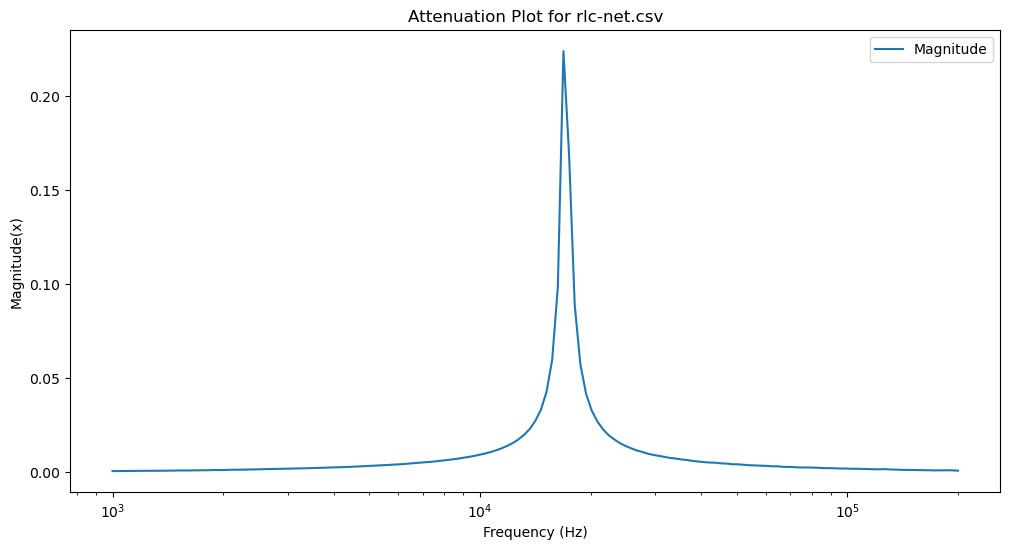
\includegraphics[width=0.7\textwidth]{Images/rlc-gain.png}
    \caption{RLC Band-Pass Gain Plot}
    \label{fig:RLC Gain Plot}
\end{figure}
\begin{table}[h!]
    \centering
    \begin{tabular}{|c|c|}
        \hline
        $f_r$ & $\Delta t$\\
        \hline
        16.57 kHz & 60.35 $\mu$s\\
        \hline
    \end{tabular}
    \caption{RLC Band-Pass Filter Ringing Frequency and $\Delta t$}
    \label{tab:RLC freq}
\end{table}
\subsection{Conclusion}
The RLC band-pass filter is a very interesting circuit. It has a very different behavior than the low and high pass filters. The ringing frequency is very interesting, and it's interesting to graphically see the band of frequencies that are able to pass through the filter. Needless to say this is very applicable in the real world, as it can be used to filter out specific frequencies from a signal, making it very versatile. This could be used in a multitude of applications, such as in radio communications, audio filters, and even in the medical field\footnote{My girlfriend actually has a hearing defect and her chochlear implant (when working) uses either a band-pass filter or a high pass filter!}.
\section{What I learned}
\begin{itemize}[label=--]
    \item The difference between a Bode plot and an Attenuation plot and how to translate between the two
    \item How to calculate the capacitance of a capacitor using the rise and fall time of a square wave
    \item How to build and analyze low, high, and band-pass filters as well as how to plot their Bode and Gain plots
    \item Gained a greated conceptual understanding of how each filter works and how voltage dividers work in general
\end{itemize}
\end{document}